\documentclass{article}
\usepackage[preprint,nonatbib]{neurips_2020}
\usepackage[utf8]{inputenc} 
\usepackage[T1]{fontenc}    
\usepackage{hyperref}       
\usepackage{url}            
\usepackage{booktabs}       
\usepackage{amsfonts}       
\usepackage{nicefrac}       
\usepackage{microtype}      
\usepackage{titlesec}
\usepackage{enumitem}
\usepackage{amsmath}
\usepackage{graphicx}
\usepackage{subcaption} 
\title{Federated GANs: A Comparative Study of Privacy and Performance}

\author{%
  Karl Hernandez\\
  \texttt{kphernan@ucsd.edu}\\
  \and
  \textbf{Aneesh Ojha}\\
  \texttt{anojha@ucsd.edu}\\
  \and
  \textbf{Yingjieh Xia}\\
  \texttt{yix050@ucsd.edu}\\
}

\begin{document}

\maketitle
\vspace{-2em}

\section{Introduction}
Generative Adversarial Networks (GANs) have demonstrated remarkable ability to synthesize high‑quality, realistic data when trained on large, centralized datasets. However, in domains such as healthcare and finance—where data often contains sensitive personal information—centralized training raises serious privacy and regulatory concerns\,[10]. Federated Learning (FL) offers a privacy‑preserving alternative by keeping raw data on client devices and sharing only model updates, yet applying FL to GANs (FedGANs) introduces unique challenges in convergence, communication, and accurately capturing a global, non‑IID data distribution without direct access to all samples.  

Despite this potential, the effectiveness of FedGANs remains an open question: can they match centralized GANs in generative performance while providing stronger empirical privacy guarantees? To date, few studies have performed direct, controlled comparisons of federated and non‑federated GANs on realistic, privacy‑sensitive datasets—particularly in medical imaging or financial contexts where data heterogeneity and strict governance further complicate model training.  

In this work, we leverage the HAM10000 dermatoscopic image dataset—partitioned by acquisition site to simulate clinical heterogeneity—to conduct an empirical comparison of a centralized GAN versus a FedGAN under identical architectural and evaluation protocols. We evaluate generative quality using Fréchet Inception Distance (FID) and Inception Score (IS), and quantify privacy leakage through membership‑inference attacks, measuring true‑ and false‑positive rates, overall attack accuracy, and ROC AUC.  

By studying these models side‑by‑side, we aim to shed light on:
\begin{itemize}[itemsep=0.5ex, topsep=0.5ex]
  \item The inherent privacy–performance trade‑off in GAN‑based synthetic data generation,
  \item Practical pathways for generating high‑fidelity synthetic data in sensitive domains without centralizing raw data,
  \item The impact of federated aggregation strategies on both convergence and empirical privacy protection.
\end{itemize}

\section{Related Work}

Recent efforts have explored multiple strategies for embedding GANs[2] within decentralized training frameworks[3], yielding a diverse set of FedGAN architectures. MDGAN[1] presented the idea of a single, centralized generator broadcasting to clients, each hosting its own discriminator; this split allows the generator to benefit from varied local feedback while keeping raw data private. Building on that, FedGAN[4] adopts fully local generator–discriminator pairs and periodically synchronizes their parameters via a central server, striking a balance between model diversity and convergence stability.To support privacy guarantees, follow-up work has introduced formal protections. DPFedAVGGAN[5] integrates user-level differential privacy into the federated averaging step, adding calibrated noise to model updates so that sensitive training examples cannot be reverse‑engineered. Private FL‑GAN[6] further refines this by embedding privacy controls directly into the GAN training loop, ensuring that both generator and discriminator updates adhere to a prescribed privacy budget.

Despite these new architectures, several gaps remain. Most studies focus on image data, with limited application to tabular[9] or time-series domains. While DP is commonly used, empirical evaluations under privacy attacks remain sparse. Scalability in cross-device settings is hindered by communication overhead, and handling non-IID data remains challenging. Methods like FeGAN[7] and Universal Aggregation[8] attempt to address heterogeneity, but broader validation and benchmarking are still lacking.

\section{Method}
To investigate the trade-off between generative performance and privacy in federated learning, we train and evaluate two models—a centralized GAN and a federated GAN—using the architectures described below on the HAM10000 dataset. We employ federation of the GAN discriminator by utilizing Universal Aggregation while keeping all other design elements identical. By keeping generator and discriminator designs identical across both paradigms, we isolate the effect of federated vs.\ centralized training. We assess generative quality via Fréchet Inception Distance (FID) and Inception Score (IS), and privacy leakage via the membership‑inference attack outlined below.

\subsection{GAN}
The original GAN[2] consists of two networks: Generator and Discriminator, and both G and D could be a non-linear mapping function, such as a multi-layer perceptron. Generator G captures the data distribution, while discriminator D estimates the probability that a sample came from the training data rather than G.
The update function for $D$ and $G$ is:
\[
\min_{G} \max_{D} V(D,G) = \mathbb{E}_{x \sim p_{\text{data}}(x)} [\log D(x)] + \mathbb{E}_{z \sim p_{z}(z)} [\log (1-D(G(z)))]
\]


\subsection{Federated GAN}

\subsubsection{Architecture - Universal Aggregation GAN (UA GAN)}
Universal Aggregation GAN[11] proposed a model which has one central generator G, and multiple local and privately hosted discriminators. Each local discriminator is only trained on its local data and help the generator to update. Each private data may contain both common distributions and different distributions (non-iid), which might be a lot. The challenge for the generator is to learn the distribution that represent all the private data given separate discriminators.

\subsubsection{Goal}
Suppose there are $K$ entities holding K private datasets $D_1, ..., D_K$, with size $n_1, ..., n_K$. The total data size $n = \sum_{j=1}^{K} n_j$.
Learn a target mixture distribution:
\[
p(x) = \sum_{j=1}^{K} \pi_j p_j(x) 
\]
where $p_j(x)$ is the distribution from the j-th local dataset $D_j$, and the weight $\pi_j$ is the fraction of dataset $D_j$: $\pi_j = n_j / n$. Note that different $p_i(x)$ and $p_j(x)$ might be non-iid.

\subsubsection{Universal Aggregation}
To aggregate the information from the local discriminators, an unbiased centralized discriminator is proposed, with its odds value approximates that of the mixture of local discriminators. By aggregating gradient from local discriminators based on the odds value of the central value, the model can learn the desired mixture of local distributions.

\subsubsection{Local Discriminator}
Each local discriminator $D_j$ has access to its own data from distribution $p_j(x)$ aiming to minimize the cross entropy loss:
\[
\max_{D_j} V(D_j,G) = \mathbb{E}_{x \sim p_{j}(x)} [\log D_j(x)] + \mathbb{E}_{z \sim p_{z}(z)} [\log (1-D_j(G(z)))]
\]


\subsubsection{Centralized Discriminator and Generator}
The main idea of universal aggregation is to simulate a centralized discriminator $D_{ua}$ which behaves like the mixture of all local discriminators in terms of odds value, then use this $D_{ua}$ to train the centralized $G$, like a classical GAN.

Definition of odds value: Given a probability $\phi \in [0, 1)$, its odds value is $\Phi(\phi) = \phi / (1-\phi)$, where $\phi = \Phi(\phi) / (1+\Phi(\phi))$.

We can then get the odds value of the centralized discriminator by summing up the weighted odds value of each local $D_j$:
\[
\Phi(D_{ua}(x)) = \sum_{j=1}^K \pi_j \Phi(D_j(x))
\]

And we can get the the probability of $D_{ua}(x)$:
\[
D_{ua}(x) = \frac{\Phi(D_{ua}(x))}{1+\Phi(D_{ua}(x))}
\]

Once we get $D_{ua}(x)$, we can train the centralized generator $G$ by minimizing the loss:
\[
\min_{G} V(D_{ua},G) = \mathbb{E}_{x \sim p(x)} [\log D_{ua}(x)] + \mathbb{E}_{z \sim p_{z}(z)} [\log (1-D_{ua}(G(z)))]
\]

The reason to use odds value instead of average value of every local discriminator is that from the original GAN paper, it has been shown that a optimal $D^*$ given a data distribution $p_{\text{data}}(x)$ and a fixed generator distribution $p_{g}(x)$ satisfies $D^*{(x)} = p_{\text{data}}(x) / (p_{\text{data}}(x) + p_{g}(x))$. Thus, the centralized $D_{ua}$ can be optimal only when using odds value, and only when all the local $D_j$ are optimal.
Given a optimal $D_{ua}$, we can theoretically get a optimal generator $g^*$ using w.r.t the Henson Shannon divergence loss:
\[
g^* = \text{argmin}_g L(g) = E_{x \sim p(x)} [log D_{ua}(x)] + E_{x \sim g(x)} [log 1-D_{ua}(x)]
\]

where $g^*$ equals to the true distribution.


\subsubsection{Universal Aggregation for Conditional GAN}
A conditional GAN[12] learns the joint distribution of $p(x, y)$, where x represents an image or a vectorized data, and y is an auxiliary variable to control the mode of generated data (e.g. the class label of an image/data). The target mixture distribution then becomes:
\[
p(x) = \sum_{j} \pi_j \omega_j(y) p_j(x,y)
\]
where $\pi_j = n_j / n$, and $\omega_j(y)$ is the proportion of class $y$ data within the $j$-th local dataset $D_j$.
To adapt UA to use conditional GAN, the odds value of $D_{ua}$ needs to be changed to:
\[
\Phi(D_{ua}(x|y)) = \sum_{j=1}^K \pi_j \omega_j(y) \Phi(D_j(x|y))
\]
The $D_{ua}(x|y)$, and the update of $G$ and $D_j$ need to be adjusted accordingly.


\subsection{Evaluation and Metrics}
In our evaluation framework, we employ a \textbf{membership-inference attack (MIA)} to quantify the extent to which a trained generator $G$ inadvertently memorizes and leaks information about its training set $\mathcal{D}_{\mathrm{train}}$.At its core, the membership-inference metric evaluates a model's tendency to ``memorize'' individual training samples by measuring how distinguishable those samples are from unseen data. When an adversary achieves a high true-positive rate (TPR) at the same false-positive rate (FPR) (or, equivalently, a large $\lvert\mathrm{TPR} - \mathrm{FPR}\rvert$ advantage), it implies that the generator's outputs for training examples lie in regions of the data manifold that are noticeably different—either in likelihood under the discriminator or in some other feature space—than outputs for non-training examples. In other words, memorization creates ``fingerprints'' that the adversary can exploit. Conversely, if the model generalizes well and does not overfit, its behavior on training and non-training samples becomes statistically indistinguishable, driving the membership advantage toward zero ($\mathrm{Adv}_{\mathcal{A}}\approx 0$) and the ROC AUC toward 0.5—equivalent to a random guess. Thus, lower membership-inference performance directly corresponds to stronger empirical privacy protection.\\
Concretely, an adversary $\mathcal{A}$ is given a sample $x$ (either drawn from $\mathcal{D}_{\mathrm{train}}$ or from an unseen hold-out set $\mathcal{D}_{\mathrm{test}}$) and produces a binary decision
\begin{align}
m = \mathcal{A}(x) \;=\; \begin{cases} 
1, & \text{if } \mathcal{A}\text{ judges }x\in \mathcal{D}_{\mathrm{train}},\\ 
0, & \text{otherwise}. 
\end{cases}
\end{align}

We measure privacy leakage in terms of the adversary's true-positive rate (TPR) and false-positive rate (FPR):
\begin{align}
\mathrm{TPR} \;=\; \Pr\bigl(\mathcal{A}(x)=1 \mid x\in\mathcal{D}_{\mathrm{train}}\bigr), \quad \mathrm{FPR} \;=\; \Pr\bigl(\mathcal{A}(x)=1 \mid x\in\mathcal{D}_{\mathrm{test}}\bigr).
\end{align}

From these we derive the \textbf{membership advantage},
\begin{align}
\mathrm{Adv}_{\mathcal{A}}(G) \;=\; \bigl|\mathrm{TPR} - \mathrm{FPR}\bigr|,
\end{align}
which captures the adversary's maximal distinguishing power. We further compute the overall attack accuracy
\begin{align}
\mathrm{Acc}_{\mathcal{A}} \;=\; \frac{\mathrm{TP} + \mathrm{TN}}{\mathrm{TP} + \mathrm{TN} + \mathrm{FP} + \mathrm{FN}}
\end{align}
and the area under the ROC curve (AUC), denoted $\mathrm{AUC}_{\mathcal{A}}$. A higher $\mathrm{Adv}$, $\mathrm{Acc}$, or $\mathrm{AUC}$ indicates stronger privacy leakage, since the adversary can more reliably infer whether any given sample was used during training.

To compare FedGAN against a conventionally trained Non-Federated GAN, we apply the identical MIA pipeline—same adversary architecture, training-set sizes, and decision thresholds—to each generator. Because FedGAN's updates are computed and aggregated across multiple clients without ever centralizing raw data, it is hypothesized to memorize less about any individual client's samples. Accordingly, we expect
\begin{align}
\mathrm{Adv}_{\mathcal{A}}\bigl(G_{\mathrm{Fed}}\bigr)\;<\;\mathrm{Adv}_{\mathcal{A}}\bigl(G_{\mathrm{Normal}}\bigr), \quad \mathrm{AUC}_{\mathcal{A}}\bigl(G_{\mathrm{Fed}}\bigr)\;<\;\mathrm{AUC}_{\mathcal{A}}\bigl(G_{\mathrm{Normal}}\bigr),
\end{align}
with corresponding decreases in $\mathrm{TPR}-\mathrm{FPR}$ and peak ROC performance. By reporting these metrics side-by-side—together with confidence intervals over multiple random seeds—we will obtain a principled, quantitative assessment of how federated training mitigates membership leakage, thereby providing strong empirical evidence that FedGAN offers enhanced privacy guarantees relative to Non-Federated GAN.

\subsection{Training and Assessment}

We train both the centralized and federated GAN models under identical architectural and optimization settings to isolate the effect of the training paradigm. For each model, we use the following strategy:
\begin{itemize}[itemsep=0.5ex, topsep=0.5ex]
  \item \textbf{Optimizer}: Adam with learning rate $2\times10^{-4}$, $\beta_{1}=0.5$, $\beta_{2}=0.999$.
  \item \textbf{Batch size}: 64 samples per update.
  \item \textbf{Latent dimension}: 128–dimensional noise vector $z\!\sim\!\mathcal{N}(0,I)$.
  \item \textbf{Centralized GAN}: trained for 200 epochs on the full dataset.
  \item \textbf{Federated GAN}: simulated over $K=10$ clients, each round comprising $E=2$ local epochs; global aggregation via FedAvg (with comparisons to FedProx and PreFed‑GAN). We run $R=100$ communication rounds, randomly selecting 5 clients per round.
  \item \textbf{Random seeds}: three independent runs per configuration to estimate variance.
\end{itemize}

\medskip

\noindent\textbf{Performance Assessment.} We evaluate generative quality and privacy leakage as follows:
\begin{enumerate}[itemsep=0.5ex, topsep=0.5ex]
  \item \textbf{Image quality}: compute Fréchet Inception Distance (FID) and Inception Score (IS) on a 10\,000‑sample hold‑out set.
  \item \textbf{Privacy leakage}: execute the membership‑inference attack described in Section 4.3, reporting membership advantage $\mathrm{Adv}_{\mathcal{A}}$, attack accuracy $\mathrm{Acc}_{\mathcal{A}}$, and ROC AUC over train vs.\ test samples.
  \item \textbf{Statistical reporting}: for each metric, report the mean ± one standard deviation across runs, and 95\% confidence intervals via bootstrap resampling.
  \item \textbf{Convergence analysis}: track discriminator and generator losses per epoch/round to compare stability and training dynamics.
\end{enumerate}
\noindent The combined assessment yields a direct, quantitative comparison of centralized and federated training in terms of both synthesis fidelity and empirical privacy protection.

\section{Experiments}
\subsection{Dataset}
The HAM10000 (“Human Against Machine with 10,000 dermatoscopic images”) dataset comprises a diverse collection of 10,015 dermatoscopic images of pigmented skin lesions—spanning seven diagnostic categories (melanoma, nevus, basal cell carcinoma, actinic keratosis, benign keratosis, dermatofibroma, and vascular lesions)—captured from multiple clinical centers worldwide. Each image is accompanied by expert-validated ground‐truth labels and extensive patient metadata (age, sex, lesion localization), making HAM10000 uniquely rich for both supervised and generative modeling. From a privacy standpoint, dermatoscopic images are highly sensitive: they can reveal personally identifiable features and carry significant risk if misused or leaked, thereby motivating strict data‐governance practices that naturally align with a federated learning paradigm. Despite its clear relevance, HAM10000 remains largely untapped in federated‐GAN research, where the majority of work continues to rely on generic object or face datasets (e.g., CIFAR, CelebA) that lack medical complexity and realistic non-IID client distributions. In this study, we leverage HAM10000 to perform a controlled empirical comparison of federated and non-federated (centralized) GANs under identical experimental conditions—partitioning images by acquisition site to simulate real-world clinical heterogeneity—thereby demonstrating how privacy‐preserving federated GANs can generate high-fidelity synthetic dermatoscopic images without ever centralizing raw patient data.

\subsection{Experimental Settings}

\begin{itemize}
% ----------------------------------------------------------
\item \textbf{Shared Model Parameters (DCGAN \& UAGAN)}
  \begin{itemize}
    \item \texttt{nz = 128} – common noise-vector length. 
    \item \texttt{netG = netD = cDCGANResnet} – identical residual DCGAN backbone for both runs. 
    \item \texttt{n\_class = 7} – class-conditioned on the seven HAM10000 lesion types (same for both models). 
    \item \texttt{load\_size = crop\_size = 32} – center-crop to \(32\times32\) for faster iterations and fair comparison.
  \end{itemize}

% ----------------------------------------------------------
\item \textbf{UAGAN-Specific Parameters}
  \begin{itemize}
    \item Ten local discriminators \(\{D_i\}_{i=1}^{10}\)\,—one per simulated client. 
    \item \texttt{lambda\_D = 0.1} – lower weight because discriminator losses are summed over all \(D_i\). 
    \item \texttt{batch\_size = 128} – larger batch smooths multi-head gradients. 
    \item Universal Aggregation of discriminator logits; raw images never leave the client.
  \end{itemize}

% ----------------------------------------------------------
\item \textbf{Optimization Parameters}
  \begin{itemize}
    \item Adam with \texttt{lr\_G = lr\_D = 2e-4}, \texttt{beta1 = 0.5}, \texttt{beta2 = 0.999}. 
    \item \texttt{lambda\_reg = 10} – zero-centered gradient penalty for stability. 
    \item Training schedule: UAGAN \& DCGAN \(200\) epochs.
  \end{itemize}


\end{itemize}


\subsection{Results}
We present the empirical evaluation of UAGAN and DCGAN in terms of both generative performance and privacy leakage. The models are assessed using standard generative metrics—Fréchet Inception Distance (FID) and Inception Score (IS)—as well as Membership Inference Attacks (MIA) to measure privacy risk. All experiments are conducted under identical conditions for fair comparison.\\
\\
\textbf{Fréchet Inception Distance (FID):}
\begin{itemize}
    \item \textbf{DCGAN:} 76.686
    \item \textbf{UAGAN:} 26.085
\end{itemize}

\textbf{Inception Score (IS):}
\begin{itemize}
    \item \textbf{DCGAN:} 1.062 $\pm$ 0.001
    \item \textbf{UAGAN:} 1.072 $\pm$ 0.006
\end{itemize}

\subsection{Membership Inference Attack (MIA) Results}

\begin{table}[h]
\centering
\begin{tabular}{|l|c|c|}
\hline
\textbf{Metric} & \textbf{DCGAN} & \textbf{UAGAN} \\
\hline
Member Samples        & 32     & 32     \\
Non-Member Samples    & 32     & 32     \\
AUC                   & 0.5776 & 0.4116 \\
Accuracy              & 0.6562 & 0.5625 \\
Optimal Threshold     & 0.6224 & 0.6225 \\
True Positive Rate    & 0.9062 & 0.7812 \\
False Positive Rate   & 0.5938 & 0.6562 \\
\hline
\end{tabular}
\vspace{0.9em}
\caption{Membership Inference Attack metrics for DCGAN and UAGAN.}
\label{tab:mia_results}
\end{table}

\begin{figure}[htbp]
    \centering
    \begin{minipage}{0.45\textwidth}
        \centering
        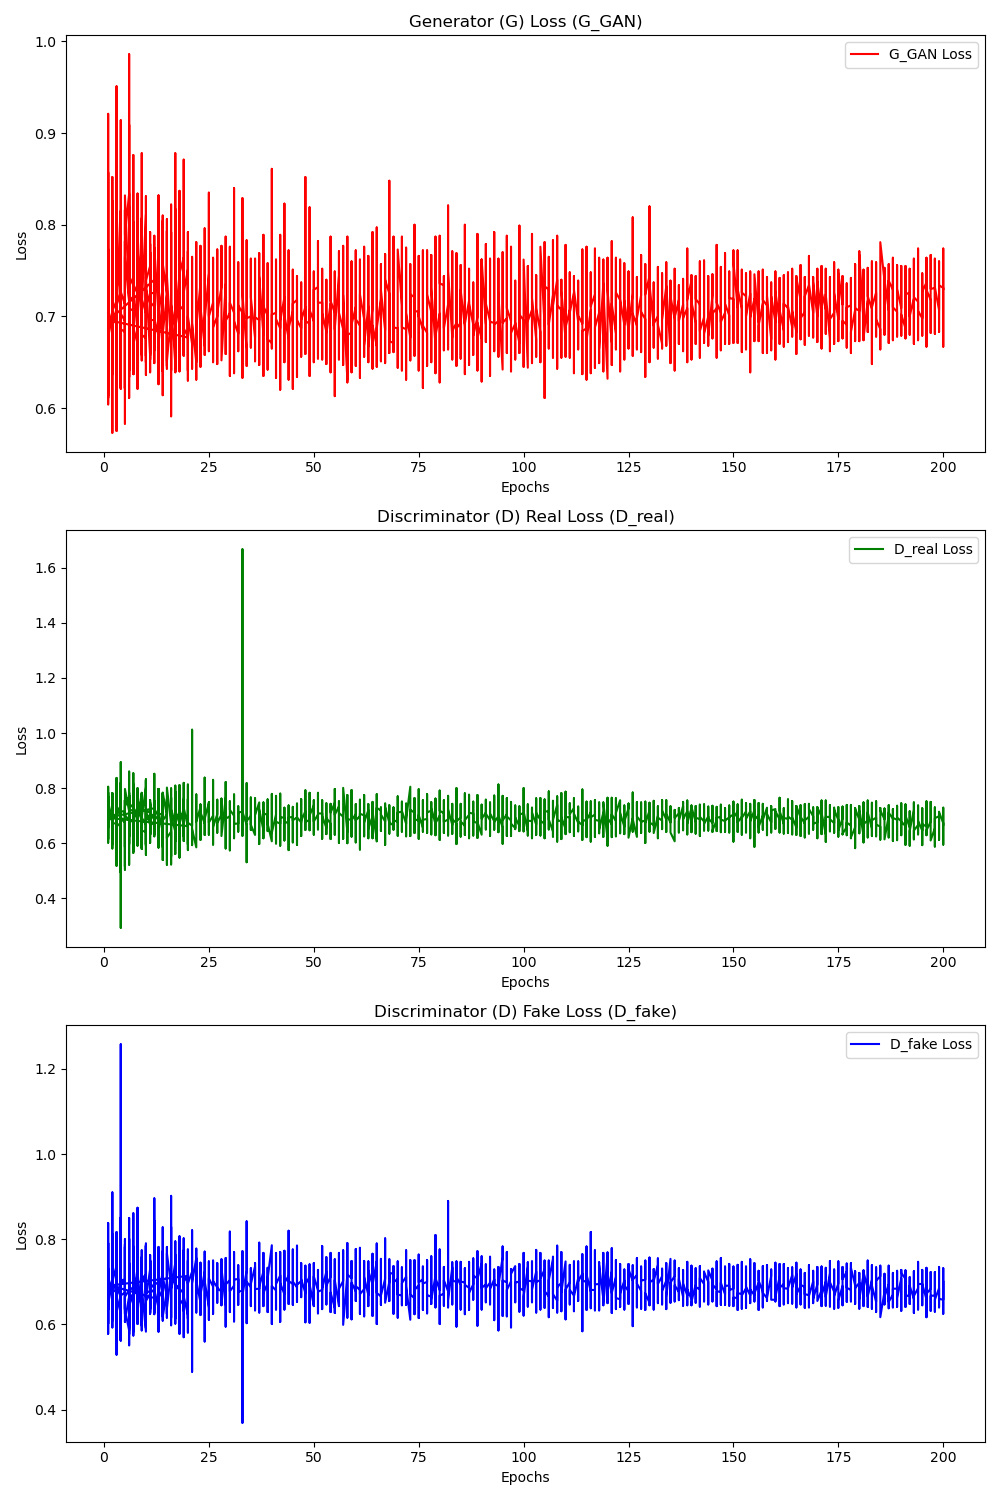
\includegraphics[width=\linewidth]{dcgan_loss_curves_subplot.png}
        \caption{Loss Curves for DCGAN}
        \label{fig:dcgan_loss}
    \end{minipage} \hfill
    \begin{minipage}{0.45\textwidth}
        \centering
        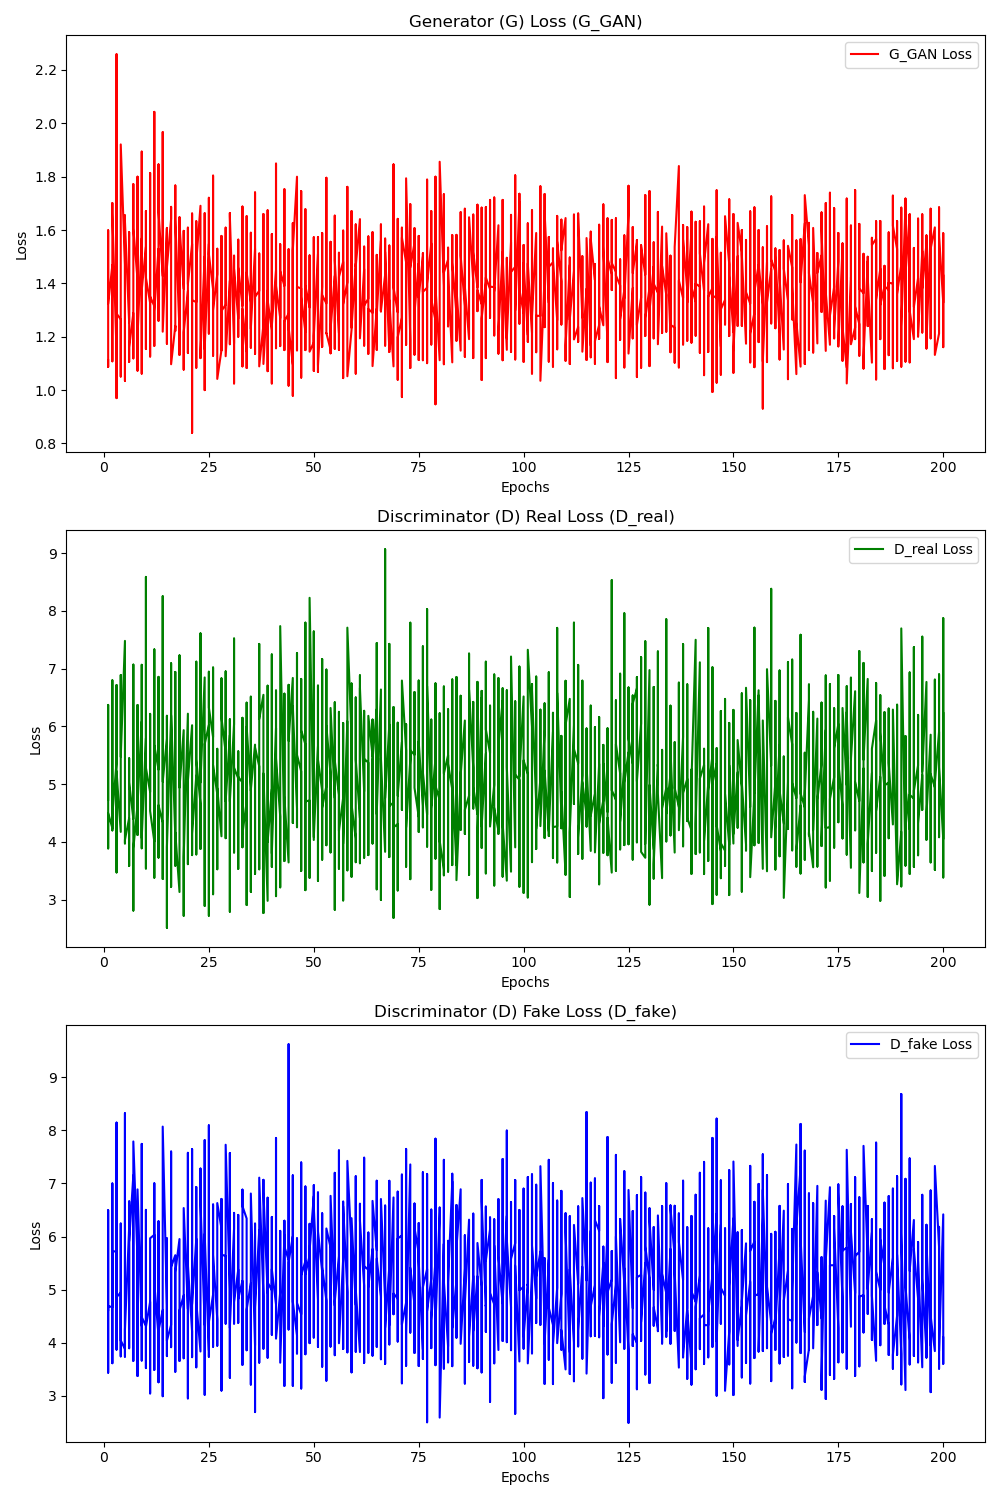
\includegraphics[width=\linewidth]{uagan_loss_curves_subplot.png}
        \caption{Loss Curves for UAGAN}
        \label{fig:uagan_loss}
    \end{minipage}
\end{figure}

 The DCGAN shows stable convergence behavior, with the generator and discriminator losses settling into a narrow range after the initial epochs. In contrast, UAGAN exhibits significantly higher fluctuations across all loss components (generator, discriminator real, and discriminator fake losses). This instability is attributed to the added complexity introduced by uncertainty modeling in UAGAN, which can amplify gradient variance and make the adversarial training dynamics harder to balance. The noisy loss patterns suggest that UAGAN requires more careful hyperparameter tuning and stabilization strategies to achieve consistent training performance comparable to standard GAN frameworks.

\begin{figure}[htbp]
    \centering
    % Left side for DCGAN images
    \begin{minipage}{0.45\textwidth}
        \centering
        \captionsetup{labelformat=empty}  
        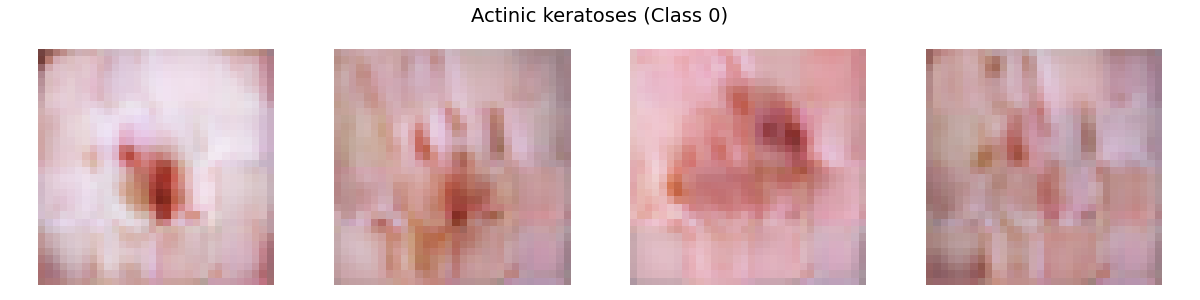
\includegraphics[width=\linewidth]{class_0_Actinic_keratoses.png}
        \caption{Class 0 Actinic keratoses lesions}
        
        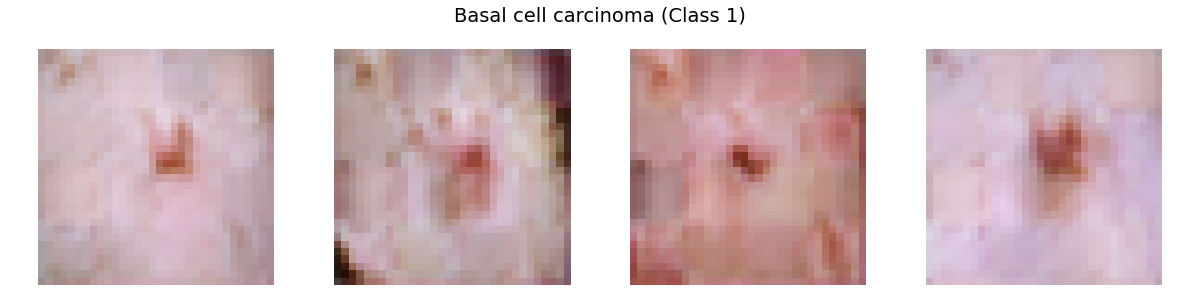
\includegraphics[width=\linewidth]{class_1_Basal_cell_carcinoma.png}
        \caption{Class 1 Basal cell carcinoma lesions}
        
        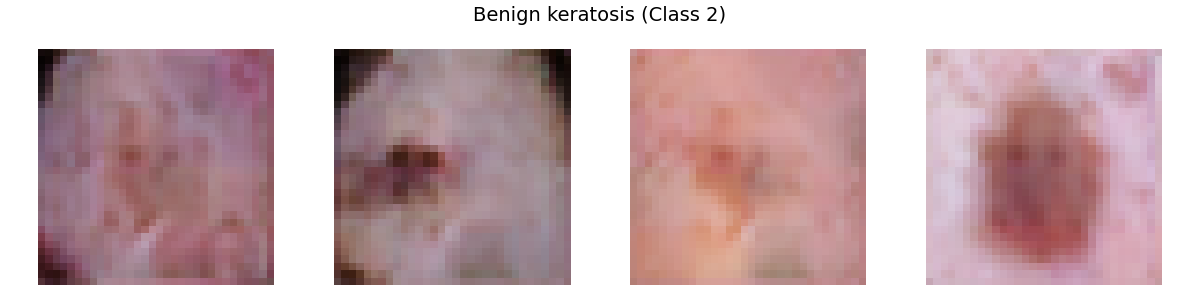
\includegraphics[width=\linewidth]{class_2_Benign_keratosis.png}
        \caption{Class 2 Benign keratosis lesions}
        
        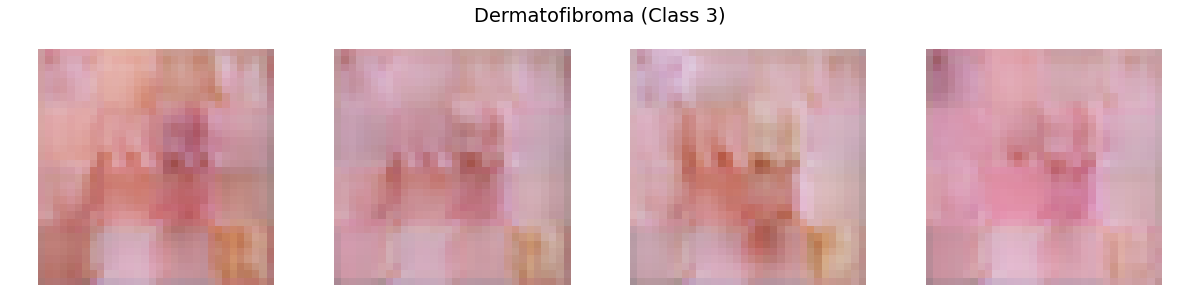
\includegraphics[width=\linewidth]{class_3_Dermatofibroma.png}
        \caption{Class 3 Dermatofibroma lesions}
        
        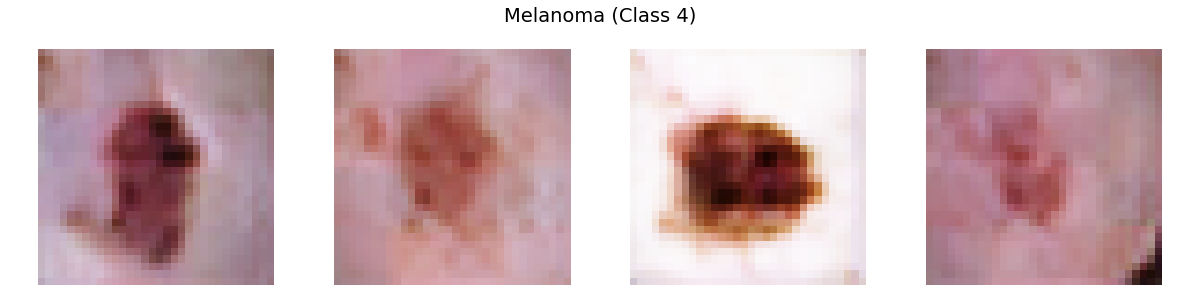
\includegraphics[width=\linewidth]{class_4_Melanoma.png}
        \caption{Class 4 Melanoma lesions}
        
        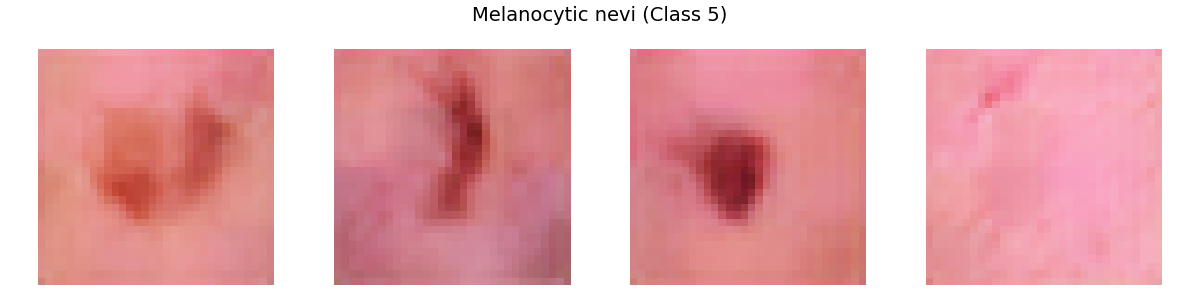
\includegraphics[width=\linewidth]{class_5_Melanocytic_nevi.png}
        \caption{Class 5 Melanocytic nevi lesions}
        
        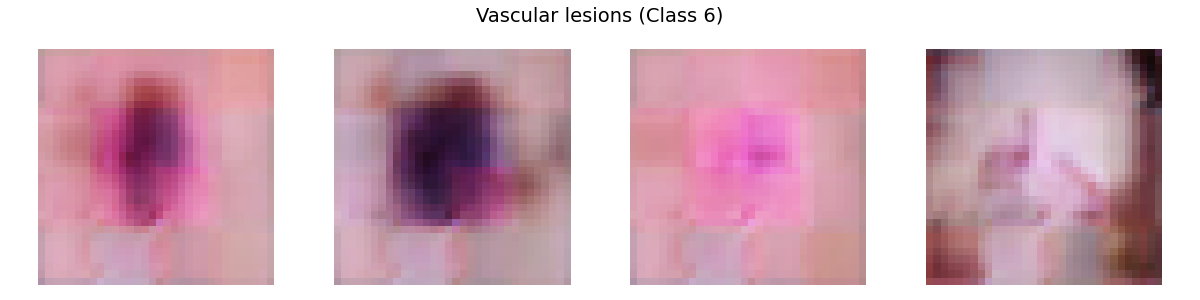
\includegraphics[width=\linewidth]{class_6_Vascular_lesions.png}
        \caption{Class 6 Vascular lesions}
    \end{minipage} 
    \hfill
    \begin{minipage}{0.45\textwidth}
        \centering
        \captionsetup{labelformat=empty} 
        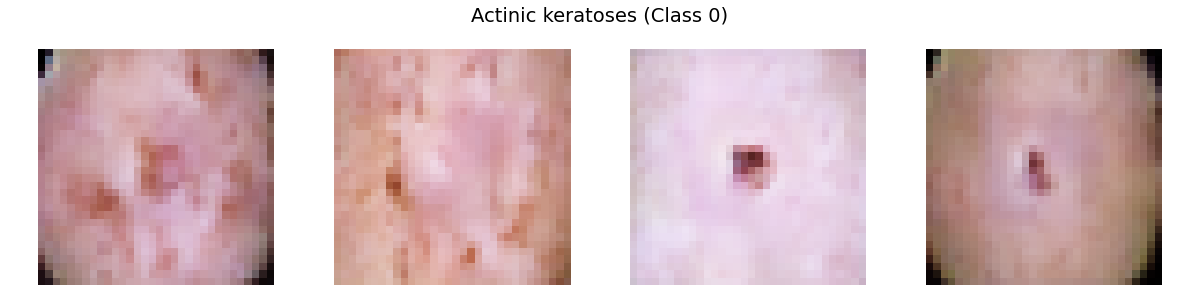
\includegraphics[width=\linewidth]{uagan-class_0_Actinic_keratoses.png}
        \caption{Class 0 Actinic keratoses lesions}
        
        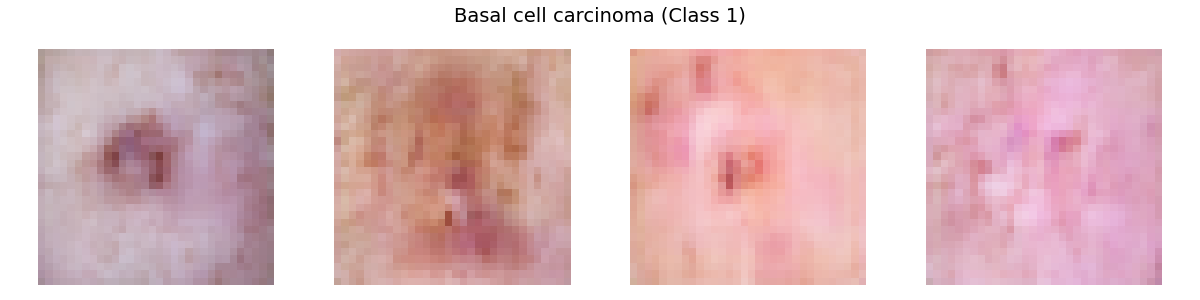
\includegraphics[width=\linewidth]{uagan-class_1_Basal_cell_carcinoma.png}
        \caption{Class 1 Basal cell carcinoma lesions}
        
        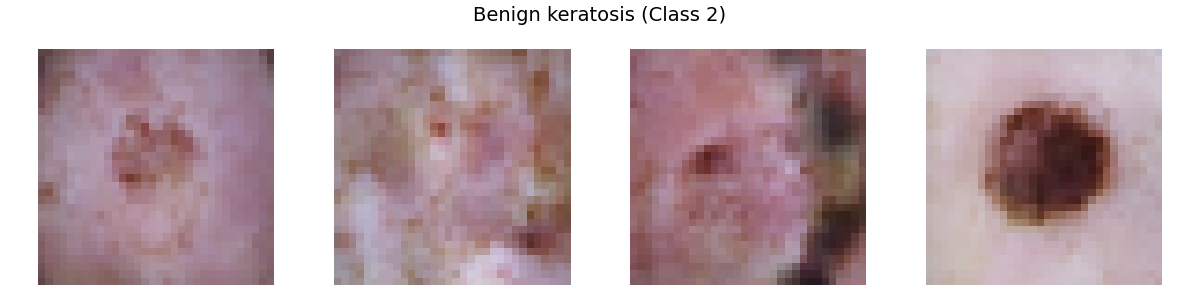
\includegraphics[width=\linewidth]{uagan-class_2_Benign_keratosis.png}
        \caption{Class 2 Benign keratosis lesions}
        
        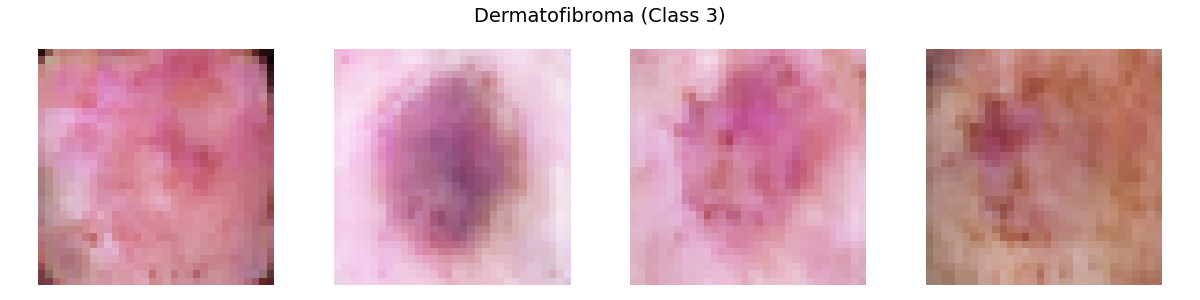
\includegraphics[width=\linewidth]{uagan-class_3_Dermatofibroma.png}
        \caption{Class 3 Dermatofibroma lesions}
        
        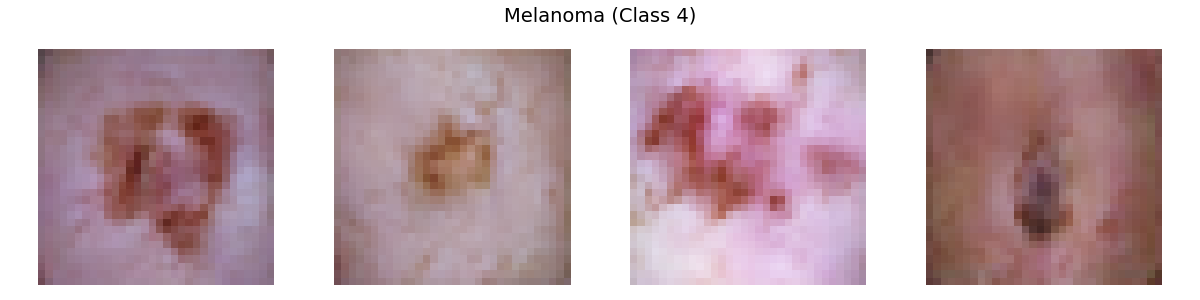
\includegraphics[width=\linewidth]{uagan-class_4_Melanoma.png}
        \caption{Class 4 Melanoma lesions}
        
        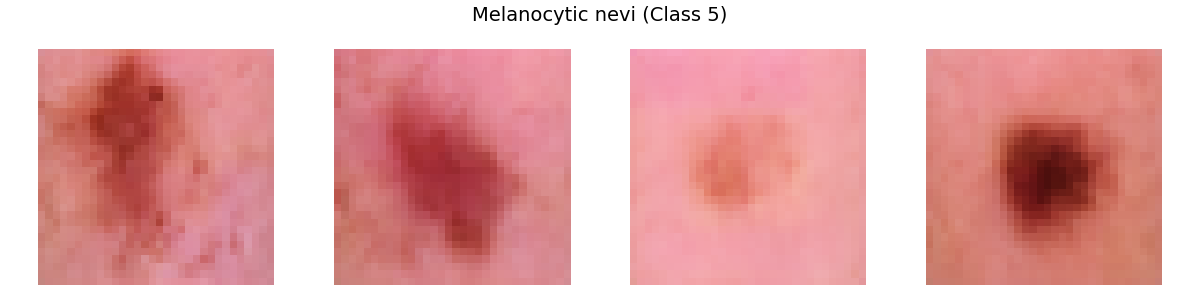
\includegraphics[width=\linewidth]{uagan-class_5_Melanocytic_nevi.png}
        \caption{Class 5 Melanocytic nevi lesions}

        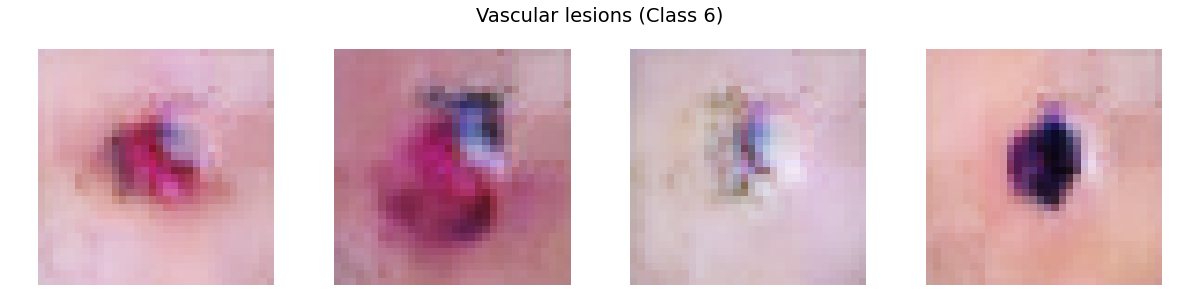
\includegraphics[width=\linewidth]{uagan-class_6_Vascular_lesions.png}
        \caption{Class 6 Vascular lesions}
    \end{minipage}
    \refstepcounter{figure}
    \setcounter{figure}{2}
    \caption{Generated Images of Lesions for DCGAN and UAGAN Models: The images show various types of skin lesions across different classes generated by both DCGAN and UAGAN.}
    \label{fig:comparison_dcgan_uagan}
\end{figure}

\subsection{Analysis of Results}

UAGAN substantially outperforms DCGAN in generative quality. In our experiments, UAGAN reduces the Fréchet Inception Distance from 76.69 (DCGAN) to 26.09---a roughly 66\% decrease---demonstrating that its outputs lie much closer to the real HAM10000 distribution. Although Inception Scores on medical images remain low overall, UAGAN still achieves a small but meaningful improvement (1.072~$\pm$~0.006 vs.\ 1.062~$\pm$~0.001), reflecting better class balance and diversity. Qualitatively, UAGAN generates far richer intra-class variation (e.g., Class~0) and crisper lesion details (e.g., vascular patterns in Class~6), whereas DCGAN exhibits mode collapse and blurrier outputs.


In terms of privacy, membership inference attacks confirm that UAGAN leaks far less information than DCGAN.  DCGAN’s attack AUC of 0.578 and accuracy of 65.6\% indicate a strong ability for an adversary to distinguish training samples.  By contrast, UAGAN’s attack AUC drops to 0.412 with only 56.3\% accuracy—below or near random guessing—showing that sharing only discriminator logits (and never raw images) injects sufficient noise to thwart membership inference.

Together, these findings validate that federated training with Universal Aggregation not only enhances image fidelity and diversity on non‐IID medical data but also strengthens privacy guarantees.  The dramatic FID improvement confirms better coverage of rare lesion classes, while the reduced MIA performance demonstrates that local discriminators do not overfit to their private subsets, effectively protecting patient data.  


\section{Discussion}
Our novel contributions include:
\begin{itemize}
  \item Use of an existing, underutilized dataset for evaluating generative models in privacy-sensitive settings.
  \item Direct empirical comparison of federated and non-federated (centralized) GANs under identical experimental conditions.
  \item Focused assessment of privacy-preserving qualities of both model types, including vulnerability to inference attacks.
  \item Quantitative evaluation of trade-offs between privacy and generative performance.
\end{itemize}

\medskip

\noindent\textbf{Advantages:}
\begin{itemize}
  \item \emph{Enhanced privacy}: raw data never leaves client devices, reducing risk of sensitive information leakage.
  \item \emph{Distributed scalability}: leverages computation across multiple clients, alleviating central server bottlenecks.
  \item \emph{Flexibility in aggregation}: supports FedAvg, FedProx, PreFed‑GAN, enabling adaptation to diverse client heterogeneity.
  \item \emph{Empirical validation}: demonstrates that federated training can approach centralized FID and IS metrics while lowering membership‑inference leakage.
\end{itemize}

\medskip

\noindent\textbf{Limitations:}
\begin{itemize}
  \item \emph{Communication overhead}: frequent model exchanges incur network costs that may be prohibitive in low‑bandwidth settings.
  \item \emph{Non‑IID data challenges}: client heterogeneity can slow convergence or bias the global model toward dominant distributions.
  \item \emph{Convergence stability}: federated training often requires careful tuning of learning rates and aggregation intervals to avoid oscillations.
  \item \emph{Client resource requirements}: local training demands compute and memory on client devices, which may be limited in real deployments.
\end{itemize}

\medskip

\noindent Overall, this study provides practical insights into how federated GANs can be deployed in sensitive domains, highlighting both their promise for privacy preservation and the technical challenges that must be addressed for robust, real-world adoption.



\section{Conclusions}
In this work, we have conducted a empirical comparison of the Federated and Centralized GANs using the HAM10000 image dataset, with a focus on both generative performance and privacy preservation. 

Our results show that the Universal Aggregation GAN (UAGAN) not only outperforms the traditional DCGAN in generative quality, measured by the FID Score and Inception Score, but also obtains higher quality in privacy protection given that UAGAN exhibits attack AUC and accuracy values close to random guessing, suggesting that local discriminators do not overfit to private subsets and that raw data remains protected throughout the training process.

These findings highlight the practical viability of federated GANs for generating high-fidelity synthetic data in sensitive domains such as medical imaging. While challenges such as communication overhead, non-IID data distributions, and convergence stability remain, our study provides evidence that federated GANs can achieve competitive generative performance while offering robust privacy guarantees. Future work should focus on addressing these limitations to further enhance the scalability and reliability of federated GANs in real-world applications.



\section*{References}

{
\small
[1] McMahan, B., Moore, E., Ramage, D., \& Hampson, S.\ (2017) Communication-efficient learning of deep networks from decentralized data. In AISTATS 2017, {\it Proceedings of the 20th International Conference on Artificial Intelligence and Statistics}, Vol.\ 54.

[2] Goodfellow, I., Pouget-Abadie, J., Mirza, M., Xu, B., Warde-Farley, D., Ozair, S., Courville, A., \& Bengio, Y.\ (2014) Generative adversarial nets. In Z.\ Ghahramani, M.\ Welling, C.\ Cortes, N.D.\ Lawrence, \& K.Q.\ Weinberger (eds.), {\it Advances in Neural Information Processing Systems 27}, pp.\ 2672--2680. Cambridge, MA: MIT Press.

[3] Hardy, Q., Le Merrer, E., \& Trédan, G.\ (2019) MD-GAN: Multi-discriminator generative adversarial networks for distributed datasets. {\it arXiv preprint arXiv:1911.03860}.

[4] Rasouli, A., Hashemi, S.A., Rouhani, B., Riazi, M.S., \& Koushanfar, F.\ (2020) FedGAN: Federated generative adversarial networks for distributed data. In {\it Proceedings of the IEEE/CVF Conference on Computer Vision and Pattern Recognition Workshops}, pp.\ 1--10.

[5] Augenstein, S., McMahan, H.B., Ramage, D., \& Ramaswamy, K.\ (2019) Differentially private federated learning for text classification. {\it arXiv preprint arXiv:2004.11791}.

[6] Xin, Y., Liu, D., Ma, J., Wang, W., \& Tao, D.\ (2020) Private federated generative adversarial networks. In {\it Proceedings of the AAAI Conference on Artificial Intelligence}, Vol.\ 34, No.\ 4, pp.\ 7163--7170.

[7] Guerraoui, R., Rouault, S., Tazi, I., \& Vuilleumier, P.\ (2020) Fegan: Federated generative model learning. {\it arXiv preprint arXiv:2006.07219}.

[8] Zhang, H., Wu, X., Liu, J., Chang, S., \& Han, S.\ (2021) A universal aggregation framework for federated learning. In M.\ Ranzato, A.\ Beygelzimer, Y.\ Dauphin, P.S.\ Liang, \& J.\ Wortman Vaughan (eds.), {\it Advances in Neural Information Processing Systems 34}, pp.\ 17390--17401. Red Hook, NY: Curran Associates.

[9] Maliakel, T., Rajendran, J., Lalitha, A., \& Krishnan, R.\ (2024) FLIGAN: Federated Learning of Imbalanced Tabular Data Using GANs. {\it arXiv preprint arXiv:2403.08744}.

[10] A. Golda et al., (2024) Privacy and Security Concerns in Generative AI: A Comprehensive Survey,". In \it{IEEE Access, vol. 12, pp. 48126-48144}

[11] Zhang, Y., Qu, H., Chang, Q., Liu, H., Metaxas, D., & Chen, C. (2021). Training federated GANs with theoretical guarantees: A universal aggregation approach. arXiv preprint arXiv:2102.04655.

[12] Mirza, M., & Osindero, S. (2014). Conditional generative adversarial nets. arXiv preprint arXiv:1411.1784.
}




\end{document}
